\documentclass{sig-alternate-05-2015}

\usepackage[utf8]{inputenc}

\title{On the security of encryption and compression composition under reflection attacks}

\numberofauthors{3}

\author{
\alignauthor
Dimitris Karakostas\\
       \affaddr{University of Athens}\\
       \email{dimit.karakostas@gmail.com}
\alignauthor
Aggelos Kiayias\\
       \affaddr{University of Athens}\\
       \email{aggelos@di.uoa.gr}
\alignauthor
Dionysis Zindros\\
       \affaddr{University of Athens}\\
       \email{dionyziz@di.uoa.gr}
}
\date{May 2016}

\usepackage{url}
\usepackage{amsmath}
\usepackage{graphicx}
\usepackage{listings}
\usepackage{mathtools}
\usepackage{amsfonts}
% \usepackage{amsthm}
\usepackage{amssymb}
\usepackage[colorlinks=true,linkcolor=blue,citecolor=green]{hyperref}

\DeclarePairedDelimiter{\ceil}{\lceil}{\rceil}
\let\oldemptyset\emptyset
\let\emptyset\varnothing

\newtheorem{lemma}{Lemma}

\newcommand\defeq{\stackrel{\mathclap{\normalfont\mbox{def}}}{=}}
\newcommand{\overbar}[1]{\mkern 1.5mu\overline{\mkern-1.5mu#1\mkern-1.5mu}\mkern 1.5mu}

\begin{document}

\maketitle

\section{Abstract}\label{sec:abstract}
When compression is composed with encryption, unexpected vulnerabilities can
arise. The information leakage through data compression was first described by
Kelsey \cite{c13} and such vulnerabilities have been explored in practical
attacks against TLS such as CRIME \cite{c1}, TIME\cite{c2} and BREACH\cite{c3}.
We introduce an abstract theoretical model for such attacks, the
\textit{adaptive reflection security} model. We discuss what properties common
compression function have, such as the \textit{compression-detectability} of
predicates, and we show that all length-preserving encryption schemes are
vulnerable when composed with such functions. Finally, we provide a modular
scalable open-source production-grade generic attack framework where these
attacks are implemented in a robust manner.

\section{Reflection security}\label{sec:refsec}

\subsection{Adaptive reflection game}\label{subsec:refsecgame}

Let $\mathcal{PE} = (\mathcal{K}, \mathcal{E}, \mathcal{D})$ be a public-key
encryption scheme, $\mathcal{A}$ be an adversary and $\mathcal{S}$ be a
simulator of $\mathcal{A}$.  The game
$\text{Game}_{\text{REF-SEC}}^{\mathcal{PE},\mathcal{A}}(\lambda,  f,
\mathcal{V}, g)$ is parameterized with a rendering function $f(\cdot, \cdot,
\cdot)$, a noise distribution $\mathcal{V}$, the security parameter $\lambda$,
some function $g$ of the plaintext, and a distribution of secrets $\mathcal{M}$
such that $\forall s \in \mathcal{M}: |s| = \lambda$.

The challenger produces a $\lambda$-bit key $(pk, sk) \leftarrow
\mathcal{K}(\lambda)$. The adversary is given $pk$, $\mathcal{V}$, $g$ and $f$.
The challenger then chooses a secret $s \leftarrow \mathcal{M}$.

The adversary is then allowed to run and make arbitrary calls to a reflection
oracle. The oracle is parameterized by $s$, the secret unknown to the
adversary.  For the reflection oracle call, the adversary chooses a reflection
string $r_i$ and sends it to the oracle. The oracle produces a noise string
$v_i \leftarrow \mathcal{V}$ and computes $m_i = f(s, r_i, v_i)$.  Subsequently
$m_i$ is encrypted as $c_i = \mathcal{E}_\kappa(m_i)$, and $c_i$ is sent back
to the adversary.

When the adversary decides to complete the game, they output a guess $y$. The
adversary is successful if $g(s) = y$.

Formally, let the public key adversarial game be defined as follows:

\begin{lstlisting}[texcl,mathescape]
def $\text{Game}_{\text{REF-SEC}}^{\mathcal{PE},\mathcal{A}}(\lambda, f, \mathcal{V}, \mathcal{M}, g)$:
    $(pk, sk) \leftarrow \mathcal{K}(\lambda)$
    $s \leftarrow \mathcal{M}$
    $y \leftarrow \mathcal{A}^{\text{Reflect}^{\mathcal{E}_{pk}, \mathcal{V}}_s(r)}(\lambda, f, \mathcal{V}, \mathcal{M}, g)$
    if $y = g(s)$:
        return 1
    else:
        return 0
\end{lstlisting}

Where the reflection oracle provided to the adversary is as follows:

\begin{lstlisting}[texcl,mathescape]
def $\text{Reflect}^{\mathcal{E}_{pk}, \mathcal{V}}_s(r)$:
    $v \leftarrow \mathcal{V}$
    $m = f(s, r, v)$
    $c \leftarrow \mathcal{E}_{pk}(m)$
    return $c$
\end{lstlisting}

Let the simulator game be defined as follows:

\begin{lstlisting}[texcl,mathescape]
def $\text{Game}_{\text{REF-SIM}}^{\mathcal{PE},\mathcal{S}}(\lambda, f, \mathcal{V}, \mathcal{M}, g)$:
    $y \leftarrow \mathcal{S}(f, \mathcal{V}, \mathcal{M}, g)$
    $s \leftarrow \mathcal{M}$
    if $y = g(s)$:
        return 1
    else:
        return 0
\end{lstlisting}

Let:

\begin{align*}
    \text{Adv}_{\mathcal{PE}, \mathcal{A}, \mathcal{S}}&(\lambda, f, \mathcal{V}, \mathcal{M}, g) &\defeq\\
    |\Pr[\text{Game}_{\text{REF-SEC}}^{\mathcal{PE},\mathcal{A}}(\lambda, f, \mathcal{V}, \mathcal{M}, g) = 1] &-\\
    \Pr[\text{Game}_{\text{REF-SIM}}^{\mathcal{PE},\mathcal{S}}(\lambda, f, \mathcal{V}, \mathcal{M}, g) = 1]| &
\end{align*}

The above game can be modified to deal with symmetric encryption. For this, the
choice of key is changed to be limited to a secret key instead of a public and
private key pair. The adversary is not given access to any key material.
Instead, the adversary is given access to an encryption oracle which encrypts a
given message using the secret key and returns the respective ciphertext, in
addition to the existing reflection oracle. Both oracles can be called an
arbitrary number of times by the challenger.

In the following proofs, we will assume that the game is played symmetrically.
As the attack does not pertain to the key exchange mechanism, all theorems can
be directly translated between the two versions of the game.

\subsection{Adaptive reflection security}\label{subsec:adaptiverefsec}

Given a polynomially computable rendering function $f(\cdot, \cdot, \cdot)$ and
a  noise distribution $\mathcal{V}$, a public-key encryption scheme
$\mathcal{PE}$ is \textit{reflection-secure} if:

\begin{align*}
\forall \mathcal{M}:
\forall g:
\forall PPT \mathcal{A}:
\exists PPT \mathcal{S}:\\
\text{Adv}_{\mathcal{PE}, \mathcal{A}, \mathcal{S}}(\lambda, f, \mathcal{V}, \mathcal{M}, g) = negl(\lambda)
\end{align*}

\section{The security of compression}\label{sec:comsec}

\subsection{Compression functions}\label{subsec:comfunc}

A compression function $Com$ is a polynomial polynomially reversible $1 - 1$
function that takes an input $x$ and outputs $y$. $x$ is a random variable that
follows the distribution $X$. $y = Com(x)$ will follow the
distribution $Com(X)$.  $E(|y|) / E(|x|) < 1$ is the metric that defines the
function's performance, where $E$ denotes expectation.

\subsection{Composing with compression}\label{subsec:comcompose}

We now shift our interest to algorithms which compose compression and
encryption.  Therefore, we treat the public-key encryption scheme above as a
composition of a compression and encryption algorithm:

\begin{equation*}
    \mathcal{E} = Enc \circ Com
\end{equation*}

$Com$ denotes a compression function as defined above, while $Enc$ denotes an
encryption function. We stress our important assumption that $Enc$ is defined
on $\{0, 1\}^*$ and not on some fixed-length input.

\subsection{Length monotonicity}\label{subsec:lenmonotone}

An important assumption for our attack is that the encryption function $Enc$ is
\textit{length monotonic}. Specifically,

\begin{equation*}
\begin{split}
\forall m_1, m_2 \in \{0, 1\}^*\\
\forall \kappa_1, \kappa_2 \in \mathcal{K}\\
|m_2| > |m_1|
\Rightarrow
|Enc_{\kappa_1}(m_2)| \geq |Enc_{\kappa_2}(m_1)|
\end{split}
\end{equation*}

If the last inequality becomes strict, we call the encryption function
\textit{strictly length monotonic}.

A practical instance of a length monotonic encryption function is AES \cite{c4}.
Stream ciphers can be treated as strictly monotonic to the bit level.

\section{Property compressibility}\label{sec:propertycom}

Let $\mathcal{M}$ be a plaintext distribution and $Q(s)$ be a predicate on the
plaintext $s \in \mathcal{M}$. Let us use $\mathcal{M}_Q$ to denote the subset
of $\mathcal{M}$ restricted over the elements for which $Q$ holds
proportionally retaining measure and assuming $\mathcal{M}_Q \neq \emptyset$
and $\mathcal{M}_{\lnot Q} \neq \emptyset$.

For the specific property $Q$ and plaintext distribution $\mathcal{M}$, define:

\begin{equation*}
    \pi \defeq max(\Pr_{s \leftarrow \mathcal{M}}[Q(s)], 1 - \Pr_{s \leftarrow \mathcal{M}}[Q(s)])
\end{equation*}

Let $\mathcal{V}$ be a noise distribution from which a pair of noises
$\overbar{v} = (v_1, v_2) \leftarrow \mathcal{V}^2$ is drawn.  Let $\overbar{r}
= (r_1, r_2) \in \mathcal{M}^2$ be a reflection string pair, $Com$ be a
compression function, $f$ be a rendering function, and let $\alpha(\lambda)$ be
a non-negligible function.

We now examine how the lengths of compressing a secret $s$ rendered with
reflection strings $r_1$ and $r_2$ respectively compare.

The predicate $Q$ partitions the set $\mathcal{M}$ into two partitions
$\mathcal{M}_Q$ and $\mathcal{M}_{\lnot Q}$. We are interested in reflection
string pairs $\overbar{r} = (r_1, r_2)$ for which the comparison direction
depends on which partition $s$ belongs to.  The direction of comparison can
also depend on a noise vector $\overbar{v}$.  If $s \in \mathcal{M}_Q$, it
should compress better when reflection $r_1$ is used as compared to when $r_2$
is used. On the contrary, if $s \in \mathcal{M}_{\lnot Q}$, the opposite
direction should occur.  If this is the case for the selected reflection pair
and noise pair, we say that $Q$ compares favourably under $\overbar{r},
\overbar{v}$:

\begin{equation*}
\begin{split}
    cpr^Q_{f, Com}(s, \overbar{r}, \overbar{v})
    \defeq\\
    \begin{cases}
        |Com(f(s, r_1, v_1))| < |Com(f(s, r_2, v_2))| &\text{ if } Q(s)\\
        |Com(f(s, r_1, v_1))| > |Com(f(s, r_2, v_2))| &\text{ otherwise}
    \end{cases}
\end{split}
\end{equation*}

The reflection pair $\overbar{r}$ \textit{detects} predicate $Q$ under
compression $Com$ rendered with rendering function $f$ over the secret
distribution $\mathcal{M}$ and the noise distribution $\mathcal{V}$ when:

\begin{align*}
    dtc(Q, \overbar{r}, f, Com, \mathcal{M}, \mathcal{V})
    \defeq\\
    \exists \alpha \text{ non-negl}:\\
    \Pr_{s \leftarrow \mathcal{M}_Q,
        s' \leftarrow \mathcal{M}_{\lnot Q},
        \overbar{v} \leftarrow \mathcal{V}^2}
        [cpr^Q_{f, Com}(s, \overbar{r}, \overbar{v}) \land
         cpr^Q_{f, Com}(s', \overbar{r}, \overbar{v})]
    \geq\\
    \pi + \alpha(\lambda)
\end{align*}

We call $Q$ \textit{compression-detectable} if a pair $\overbar{r}$ exists,
such that:

\begin{equation*}
    \exists \overbar{r} = r_1, r_2 \in \mathcal{M}:
    dct(Q, \overbar{r}, f, Com, \mathcal{M}, \mathcal{V})
\end{equation*}

Furthermore we require that such a pair $\overbar{r}$ is polynomially
computable:

\begin{align*}
    \exists \text{PPT } \mathcal{O}_R:\\
    dct(Q, \overbar{r}, f, Com, \mathcal{M}, \mathcal{V}),\\
    \overbar{r} \leftarrow \mathcal{O}_R(Com, f, Q, \mathcal{M}, \mathcal{V})
\end{align*}

The compression-detectability property exists in all common compression
functions as long as $s$ and $r$ compress in the same context. We will
illustrate such examples later in this work.

\section{The BREACH model}\label{sec:breachmodel}
We now turn our attention to the BREACH attack specifically, which utilizes
the properties explored above, and we show that, under ideal modeling,
the above attack is instantiated when the TLS algorithms are in use.

In the BREACH model, we deal with a specific function $f$, property $Q$,
compression function $Com$, length-leaking $Enc$, and secret distribution
$\mathcal{M}$.

In the next paragraphs, we describe a simplified model of the attack that
lends itself to formal theoretical proofs, while abstracting away the complex
practical details of the attack pertaining to the networking and particularities
of the implementation that are of little significance to the cryptographic
formalisms presented here.

\subsection{The rendering context assumption}\label{subsec:rendering}

In the modern web, function $f$ represents a specific attack target, which
constitutes the renderer of a web page, given a specific secret, reflection,
and noise. Typically, $f$ will concatenate instances of the secret, the
reflection, and the noise, between some context strings which constitute the
static portions of the site.

We assume that $f$ outputs a concatenation of various instances of $s$, $r$,
and $v$ with arbitrary repetitions, in addition to concatenating with some
constant context whose position is independent of the values of $s, r, v$.  The
number of repetitions of $s, r, v$ are also independent of the values of $s, r,
v$.

Formally, assume that the symbols $\{\beta_1, \beta_2, \beta_3\}$ do not appear
in the alphabet of the secret.

Our assumptions for $f$ can be stated as follows. Let

\begin{equation*}
\begin{split}
\exists \mu \in \{0, 1, \beta_1, \beta_2, \beta_3\}^*\\
\exists u_1, v_1, u_2, v_2, u_3, v_3 \in \{0, 1, \beta_1, \beta_2, \beta_3\}^*\\
\mu = u_1 \beta_1 v_1 \land\\
\mu = u_2 \beta_2 v_2 \land\\
\mu = u_3 \beta_3 v_3 \land\\
\forall s, r, v \in \{0, 1\}^*\\
f(s, r, v) = Rep(Rep(Rep(\mu, \beta_1, s), \beta_2, r), \beta_3, v)
\end{split}
\end{equation*}

Where $Rep$ is the string replacement function:

\begin{align*}
Rep(\epsilon, \alpha, \beta) &\defeq \epsilon\\
Rep(\alpha:xs, \alpha, \beta) &\defeq \beta:Rep(xs, \alpha, \beta)\\
Rep(x:xs, \alpha, \beta) &\defeq x:Rep(xs, \alpha, \beta)
\end{align*}

Where $:$ denotes the concatenation of a symbol with a string.

We call $f$ functions that exhibit such behavior \textit{concatenative}.

\subsection{The compression function assumption}\label{subsec:comfuncassumption}

In BREACH, $Com$ is a variant of LZ77 \cite{c5}. In this compression algorithm,
repetitions of strings are well-compressed. In our ideal model, we examine a
simplified version of LZ77 which we describe in this paragraph.

Our version of LZ77 is not composed with a symbol-compressing algorithm such as
Huffman coding. Therefore, a way is needed to encode literal symbols and
compression symbols. The LZ77 algorithm treats the uncompressed text as a
series of bits. Let the plaintext be $p$ and its length be $n = |p|$. The LZ77
compression function needs to have an alphabet of 2 symbols for representing
literals (the bits $0$ and $1$ of the plaintext) as well as an alphabet of an
additional $n$ symbols for representing compression distances from $1$ to $n$
and lengths from $1$ to $n$ (the same symbol is used to represent a distance
and a length). This makes an alphabet of a total of $n + 2$ symbols which are
represented by bit sequences of exactly $\ceil{lg(n + 2)}$ bits each.

We first describe the decompression algorithm. At the beginning of the
compressed string, the number of characters in the uncompressed plaintext is
encoded in ASCII followed by the "$\$$" ASCII character as a separator. This
allows the decoder to compute how many bits are used to represent each symbol
in the compressed text.

Ordering these bit strings lexicographically, the first two bit strings will
correspond to the literal "$0$" and "$1$" bits of the plaintext. The next bit
strings will correspond to \textit{distance} bit sequences of values $1, 2,
\ldots, n$ respectively.

After the "$\$$" separator, an encoding of the plaintext is given. The encoding
can be decompressed by linearly reading it one character at a time. If a bit
sequence corresponding to a literal is given, this is decoded as the respective
literal bit of the plaintext. If a distance bit sequence of value $a$ is given,
then another distance bit sequence of value $b$ sequence follows.  Then $a$
must be less than or equal to the plaintext characters decoded so far, while
$b$ is arbitrary. This pair of values is decoded as follows. The decompressed
text beginning at a distance of $a$ bits behind the current position decoding
position and of length $b$ bits is taken into account. That text is then the
new decompressed plaintext which is appended to the existing decompressed
plaintext one bit at a time. This procedure can cause self-overlapping texts.
In the end, the decoded text must be $n$ bits long, otherwise the compression
is invalid.

\begin{lstlisting}[texcl,mathescape]
def $\text{LZ77}^{-1}(c)$:
    parts = c.split("$\$$")
    plaintextLength = parse_int(parts[0])
    bitsPerSymbol = $\ceil{lg(\text{plaintextLength}) + 2}$
    enc = strToBinArray("".join(parts[1:]))

    plaintext = ''
    for i in range(0, len(enc), bits):
        symbol = binaryToInt(enc[i:bits])
        if symbol = 0:
            plaintext += '0'
        else if symbol = 1:
            plaintext += '1'
        else:
            d = symbol - 1
            i += bits
            length = int(enc[i:bits])
            if d > len(plaintext):
                return $\bot$
            while length:
                plaintext += plaintext[-d]
                length -= 1
    if len(plaintext) != plaintextLength:
        return $\bot$
    else:
        return plaintext
\end{lstlisting}

Where negative and range array indexing and the $range$ function is as in
Python.

Our LZ77 compressor can then be described simply: It chooses the shortest in
bits compressed text, which, when decoded using the above algorithm yields the
desired plaintext.

% TODO: Prove that it is a compression function for some $\mathcal{M}$

\subsection{The full-text predicate assumption}\label{subsec:fulltextassumption}

The BREACH attack is a specific instance of reflection-based attacks in which
the $Q$ property pertains to a prefix of the secret. It asks "Does the secret
begin with such text?"

We require $X$ to be of compressible length,
i.e. the following equation must be satisfied:

\begin{equation*}
    |X| > \ceil{lg(f(X, X, \epsilon) + 2)}
\end{equation*}

In practical terms, this requires the secret that needs to be stolen to be at
least 3 bytes so that it is better compressed rather than represented as a
literal.

\subsection{Prefixes are
compression-detectable}\label{subsec:breachprefix}

Let $startswith(v, s)$ be the $k$-length prefix checking predicate on a
$\lambda$-bit secret $s$:

\begin{equation*}
    startswith(v, s) \defeq \exists w: s = v w
\end{equation*}

\begin{lemma}

Let $f$ be a concatenative rendering function and let $Com = LZ77$. Then:

\begin{align*}
\Pr[startswith(v, \cdot) \textrm{ compression-detectable under } f, Com] =\\ \text{non-negl}(\lambda - k)
\end{align*}

Where the probability randomness is taken uniformly over all $k$-bit prefixes $v \in \{0, 1\}^k$.

\end{lemma}

\begin{proof}
?
\end{proof}

\section{Compression distinguishing attacks}\label{sec:comattack}

\begin{lemma}[Compression attack]

Let $Com$ be a compression function, $Enc$ be a strictly length-monotonic
encryption function, $f$ be a rendering function and $Q$ be a
compression-detectable plaintext predicate over plaintext distribution
$\mathcal{M}$ and noise distribution $\mathcal{V}$.

Then:

\begin{align*}
    \exists \alpha \text{ non-negl}:
    \forall Enc:
    \exists g:\\
    \exists PPT \mathcal{A}:
    \forall PPT \mathcal{S}:\\
    \text{Adv}_{\mathcal{SE}(Enc, Com), \mathcal{A}, \mathcal{S}}
    (\lambda, f, \mathcal{V}, \mathcal{M}, g) = \alpha(\lambda)
\end{align*}

\end{lemma}

\begin{proof}

Let $g$ be the boolean function $Q$ on the plaintext. Define the adversary
$\mathcal{A}$ as follows:

\begin{lstlisting}[texcl,mathescape]
def $\mathcal{A}(Q, \mathcal{M}, y)$:
    $(r_1, r_2) \leftarrow \mathcal{O}_R(Com, f, Q, \mathcal{M}, \mathcal{V})$

    $l_1 = |\text{Reflect}^{\mathcal{E}_{pk}, \mathcal{V}}_s(r_1)|$
    $l_2 = |\text{Reflect}^{\mathcal{E}_{pk}, \mathcal{V}}_s(r_2)|$

    if $l_1 < l_2$:
        return True
    else:
        return False
\end{lstlisting}

Let $\mathcal{S}$ be an arbitrary simulator. Then we have:

\begin{align*}
    \Pr[\text{Game}_{\text{REF-SIM}}^{\mathcal{PE},\mathcal{S}}
        (\lambda, f, \mathcal{V}, \mathcal{M}, g) = 1] &=\\
    \Pr_{x \leftarrow \mathcal{M}, b \leftarrow \mathcal{S}(f, \mathcal{V}, \mathcal{M}, g)}
        [Q(x) = b]
\end{align*}

Letting the random variables $b$ and $x$:

\begin{align*}
    x &\leftarrow \mathcal{M}\\
    b &\leftarrow \mathcal{S}(f, \mathcal{V}, \mathcal{M}, g)
\end{align*}

Due to the independence of the simulator's output with the choice of $x$ we have:

\begin{align*}
    Pr[b = Q(x)] &=\\
    Pr[\lnot b|\lnot Q(x)]Pr[\lnot Q(x)] + Pr[b|Q(x)]Pr[Q(x)] &=\\
    Pr[\lnot b]Pr[\lnot Q(x)] + Pr[b]Pr[Q(x)] &=\\
    (1 - Pr[b])(1 - Pr[Q]) + Pr[b]Pr[Q(x)] &=\\
    1 - Pr[Q(x)] - Pr[b] + 2Pr[b]Pr[Q(x)]
\end{align*}

For a given $\Pr[Q]$, this function is monotonic in $\Pr[b]$ and therefore has
potential extrema at $\Pr[b] = 0$ or $\Pr[b] = 1$, for which cases the function
takes the values $1 - \Pr[Q(x)]$ and $\Pr[Q(x)]$ respectively. Therefore, the
maximum $\Pr[b]$ of the simulator is:

\begin{equation*}
    \Pr[Q(x) = b] = max(\Pr[Q(x)], 1 - \Pr[Q(x)]) = \pi
\end{equation*}

And therefore:

\begin{align*}
    \forall \mathcal{S}:\\
    \Pr[
        \text{Game}_{\text{REF-SIM}}^{\mathcal{PE},\mathcal{S}}
        (\lambda, f, \mathcal{V}, \mathcal{M}, g) = 1
    ]
    \leq\\
    max(Pr[Q(x)], 1 - Pr[Q(x)])
\end{align*}

From the compression detectability of Q we know that:

\begin{align*}
    \exists \alpha \text{ non-negl}:\\
    \Pr_{s \leftarrow \mathcal{M}_Q,
         s' \leftarrow \mathcal{M}_{\lnot Q},
         \overbar{v} \leftarrow \mathcal{V}^2}
         [cpr^Q_{f, Com}(s, \overbar{r}, \overbar{v}) \land
          cpr^Q_{f, Com}(s', \overbar{r}, \overbar{v})]
    \geq\\
    \pi + \alpha(\lambda)
\end{align*}

Therefore:

\begin{align*}
    \Pr_{s \leftarrow \mathcal{M}_Q,
         \overbar{v} \leftarrow \mathcal{V}^2}
         [cpr^Q_{f, Com}(s, \overbar{r}, \overbar{v})]
    \geq
    \pi + \alpha(\lambda) \land\\
    \Pr_{s' \leftarrow \mathcal{M}_{\lnot Q},
         \overbar{v} \leftarrow \mathcal{V}^2}
         [cpr^Q_{f, Com}(s', \overbar{r}, \overbar{v})]
    \geq
    \pi + \alpha(\lambda)
\end{align*}

And so:

\begin{align*}
    \Pr_{s \leftarrow \mathcal{M},
         \overbar{v} \leftarrow \mathcal{V}^2}
         [cpr^Q_{f, Com}(s, \overbar{r}, \overbar{v})]
    =\\
    \Pr[cpr^Q_{f, Com}(s, \overbar{r}, \overbar{v})|Q(s)]\Pr[Q(s)]
    +\\
    \Pr[cpr^Q_{f, Com}(s, \overbar{r}, \overbar{v})|\lnot Q(s)]\Pr[\lnot Q(s)]
    \geq\\
    (\pi + \alpha(\lambda))(\Pr[Q(s)] + (1 - \Pr[Q(s)))
    =\\
    \pi + \alpha(\lambda)
\end{align*}

Let us now examine the event of $\mathcal{A}$ being successful, denoted Succ,
when $cpr^Q_{f, Com}(s, \overbar{r}, \overbar{v})$. Indeed:

\begin{align*}
    \Pr[|Com(f(s, r_1, v_1))| < |Com(f(s, r_2, v_2))||Q(s)]
    = \pi + \alpha(\lambda)
\end{align*}

And from the strict length monotonicity of $Enc$ it follows that:

\begin{align*}
    \Pr[&|Enc(Com(f(s, r_1, v_1)))| <\\&|Enc(Com(f(s, r_2, v_2)))||Q(s)]
        \geq \pi + \alpha(\lambda)\\
    \Rightarrow \Pr[&
        |\text{Reflect}^{\mathcal{E}_{pk}, \mathcal{V}}_s(r_1)|
        <
        |\text{Reflect}^{\mathcal{E}_{pk}, \mathcal{V}}_s(r_2)||Q(s)
    ]
        \geq \pi + \alpha(\lambda)\\
    \Rightarrow \Pr[&l_1 < l_2|Q(s)]
        \geq \pi + \alpha(\lambda)\\
    \Rightarrow \Pr[&\text{Succ}|Q(s)]
        \geq \pi + \alpha(\lambda)\\
\end{align*}

The case for $\lnot Q(s)$ is the same, but with a different inequality direction:

\begin{align*}
    \Pr[|Com(f(s, r_1, v_1))| > |Com(f(s, r_2, v_2))||Q(s)]
        \geq\\
        \pi + \alpha(\lambda)\\
    \Rightarrow \Pr[\text{Succ}|\lnot Q(s)] \geq\\
    \pi + \alpha(\lambda)\\
\end{align*}

And so the probability of success is given:

\begin{align*}
    \Pr[\text{Succ}] =\\
    \Pr[\text{Succ}|Q(s)]\Pr[Q(s)]
    +
    \Pr[\text{Succ}|\lnot Q(s)]\Pr[\lnot Q(s)] \geq\\
    \pi + \alpha(\lambda)
\end{align*}

Therefore,

\begin{align*}
    \forall PPT \mathcal{S}:
    \text{Adv}_{\mathcal{SE}(Enc, Com), \mathcal{A}, \mathcal{S}}
        (\lambda, f, \mathcal{V}, \mathcal{M}, g)
    \geq\\
    |\pi + \alpha(\lambda) - \pi| = \alpha(\lambda)
\end{align*}

Which is non-negligible.

\end{proof}

We can now amplify the attack to achieve a better probability of success by a
small modification in our adversary. The amplification is parameterized by a
parameter $k$.

\begin{lstlisting}[texcl,mathescape]
def $\mathcal{A}(Q, \mathcal{M})$:
    $(r_1, r_2) \leftarrow \mathcal{O}_R(Com, f, Q, \mathcal{M}, \mathcal{V})$

    $low = 0$
    $high = 0$

    for $i$ = $0$ to $k$:
        $l_1 = |\text{Reflect}^{\mathcal{E}_{pk}, \mathcal{V}}_s(r_1)|$
        $l_2 = |\text{Reflect}^{\mathcal{E}_{pk}, \mathcal{V}}_s(r_2)|$

        if $l_1 < l_2$:
            $low = low + 1$
        else:
            $high = high + 1$

    if $low > high$:
        return True
    else:
        return False
\end{lstlisting}

Proof that this amplifies?

\subsection{Compression is insecure}\label{subsec:cominsecure}

We now show that all reasonable compression function expose a
compression-detectable property $Q$. Indeed, if a compression function does not
expose any compression-detectable properties $Q$, then the compression function
does not cross-compress the data in $X$ with the data in $Y$ (Why?).

\section{Defense}\label{sec:defense}

Defense against side-channel compression attacks and especially BREACH have been
proposed in bibliography, including the original BREACH paper,
\cite{c6} and \cite{c7}.

\subsection{Disabling compression}\label{subsec:disablecom}
Compression is the basic assumption for property compressibility. Disabling
compression would break the adaptive reflection game, since it removes
the compression part of the encryption function.

However, this method is not viable, since the performance overhead should it be
applied overrules the benefits of the defense.

\subsection{SameSite cookies}\label{subsec:samesite}
SameSite cookies \cite{c8} is a proposed draft for enhancing web security. The
main puprose of this technique is to mitigate cross-site request forgery
attacks, although it also mitigates other kinds of cross-origin leakages.

This policy introduces a new attribute for web cookies that web servers may
opt-in. This attribute states that cookies may only be included in a
"first-party" context, i.e. in same origin requests.

However, the current BREACH application depends on cross-origin requests in
order to call the reflection oracle, as defined in \ref{subsec:breachapp}.
Enabling SameSite cookies would result in the elimination of this reflection
oracle of the Reflection-Security Game and the effective mitigation of the
attack.

\subsection{Masking secrets}\label{subsec:masking}
Masking is a method of hiding secrets' properties per request. A mask is a
bitstream equal in size with the secret. The masked text contains the result of
the XOR operation between the secret and the mask concatenated with the mask.
The secret can be obtained by applying XOR between the first and the second
half of the masked text.

A masking function is defined:

\begin{lstlisting}[texcl,mathescape]
def masking($s_i$):
    $l = |s_i|$
    $m_i \xleftarrow{\$} \{0, 1\}^l\\$
    $s_i' = m_i \oplus s$
    return $s_i', m_i$
\end{lstlisting}

Masking can be applied on a rendered secret $s_i$ in the output $m$ of a
rendering function $f$ as:

\begin{lstlisting}[texcl,mathescape]
def apply_masking($m_i, s_i$):
    $s_i', m_i \leftarrow masking(s_i)$
    return $Rep(m, s_i, \beta_1 s_i' \beta_2 m_i \beta_3)$
\end{lstlisting}

where $Rep$ is the string replacement function defined in
\ref{subsec:rendering} and $\{\beta_1, \beta_2, \beta_3\}$ are symbols that do not
appear in $m$ before masking.

Mask removal should be applied on all masked secrets, marked by the annotation
symbols $\beta_1$, $\beta_2$, $\beta_3$, before the reversing of rendering function $f$:

\begin{lstlisting}[texcl,mathescape]
def remove_masking($m', \beta_1, \beta_2, \beta_3$):
    return $Rep(m', \beta_1 s_i' \beta_2 m_i \beta_3, s_i' \oplus m_i)$
\end{lstlisting}

where $Rep$ is the string replacement function and $\{\beta_1, \beta_2,
\beta_3\}$ are the annotation symbols used in \texttt{apply\_masking}.

Mask $m_i$ is chosen uniformly at random, so masked secret $s_i'$ is also
random. This results in $s_i' m_i$ being indistinguishable from $r_1 r_2$ by a
compression function $Com$, where $r_1$, $r_2$ are random nonces chosen
uniformly at random.

Masking renews the secret $s_i'$ each time the reflection oracle is called. That
way, this method secures the secret's content against instances of the attack
that require at least two calls to the reflection oracle.

Masking doubles the size of the secret that is being protected. Furthermore,
$m_i$ and $s_i'$ are random, so the compression performance is poor. Therefore,
masking should be applied with limitation on high value secrets only, in order
to avoid significant performance drop.

Masking is a method used by Facebook \cite{c9} in order to protect CSRF tokens
against BREACH attacks.

\section{Application}\label{sec:application}

BREACH is an example of a side-channel attack, that uses reflection in
order to steal plaintext compressed and encrypted in the web.

\subsection{BREACH as a compression distinguishing
attack}\label{subsec:breachapp}
BREACH is an instance of the attack model described in \ref{sec:comattack}.

A secret is defined as any string in the response plaintext of a web page, such
as authentication tokens, private messages etc.

The property $g$ of the secret that is being compromised is defined as: "What is
the prefix $p$ of secret $s$, given a known prefix $p_s$, where $|p| - |p_s| =
1$?".

The distribution $\mathcal{M}$ is ${p_s:t}$, where $t \in \mathcal{S}$ and
$\mathcal{S}$ is a known alphabet of ASCII symbols.

The rendering function $f$ is the website response code rendering function. This
function concatenates secret $s$ with static strings $u$, noise $v$ and the
reflection string $r$.

The compression function is gzip, which implements the DEFLATE algorithm
\cite{c10}, that is the combination of LZ77 and Huffman coding.

The encryption function is any encryption algorithm used in communications over
the Internet, most notably AES.

The web application that is being attacked with BREACH offers an endpoint that
allows requests via GET, where a GET parameter is included in the response. This
endpoint constitutes the reflection oracle.

The adversary should be able to issue requests to the given endpoint and monitor
the traffic from and to the attacking browser. At this point, the adversary can
issue requests on different elements of $\mathcal{S}$ and compare the response lengths. As
long as a difference in lengths across different requests is noticeable, the
compression distinguishing attack is successful.

\subsection{Rupture implementation}\label{subsec:rupture}
Our contributions include the development development of a production-grade
framework for implementing this class of attacks called Rupture \cite{c11}.
Rupture was developed as part of the work on extending the BREACH attack against
modern systems and block ciphers and was first discussed as an attack mechanism
in \cite{c12}.

As long as a vulnerable endpoint described in \ref{sec:comattack} is found,
Rupture offers the ability to inject malicious code in any computer in the
network. This code would issue requests to the endpoint and serve as a caller of
the reflection oracle that is the endpoint.

Furthermore, it enables the traffic inspection and analysis of packet
lengths. Encrypted network packets serve as the response $c_i$ from the
reflection oracle and the length of each packet is visible on the network and
captured.

In addition, Rupture offers multiple instances of oracle $\mathcal{O}_R$, based
on various $Q$ described in \ref{subsec:parallel}, and enables the automated
computation of the reflection strings in each stage of the attack.

Finally, it amplifies the attack by issuing multiple requests per candidate
symbol in alphabet $\mathcal{S}$ in order to demonstrate better probability of
success. This is achieved by grouping requests in samplesets, where each
sampleset contains requests on a symbol in alphabet $\mathcal{S}$. Requests in a
sampleset may be constructed to enable optimization methods described in
\ref{subsec:blockalign} and \ref{subsec:parallel}.

Rupture issues the attack in rounds. Each round consists of phases, whose result
leads to the detection of property $Q$, where $Q$ is specified by the method of
attack described in \ref{subsec:parallel}, with some confidence $n$. Confidence
is a metric calculated in bytes, that depicts the length difference between a
pair $r_1, r_2$ of requests that make property $Q$ of secret $s$ compression
detectable.

\subsection{Rupture architecture}\label{app:rupture}
Rupture consists of multiple components that collaborate in executing
compression-based attacks, such as BREACH. Each component is autonomous and
communicates with the rest over the network.

The client component is a Javascript code that issues requests towards a chosen
endpoint. This endpoint should offer the functionality described in
{subsec:breachapp} and serve as the reflection oracle of the attack. The client
needs to be executed from the browser of the victim that the adversary is trying
to steal secrets from. That way, the victim's authentication cookies will be
included in the request and lead to the endpoint including secrets in the
response.

In order for the client code to run in the victim's browser, the victim should
run HTML code that includes the client script. One way is to visit a website
controlled by the adversary that has added the code. The injector component of
Rupture offers a second way. It injects the client code in the plaintext of
victim's unencrypted, unauthenticated HTTP responses and attack requests are
issued any time the victim visits a plain HTTP website and the malicious code is
injected. In order for the injection to be performed, the adversary should be
able to view and alter the victim's network traffic.

The response packets from the endpoint to the victim contain the encrypted
compressed rendering of the web page that contains both the secret and the
reflection. The sniffer component has access to the victim's network traffic and
keeps track of the encrypted communication between the victim and the endpoint.
The length of the packets is unencrypted, so the sniffer is able to collenct and
report the observations on the network to the backend component.

The backend component is a Python code that controls the attack execution. It
initializes the attack and calculates the initial request sets that should be
collected. It communicates with the realtime component in order to guide the
client as to what requests need to be made at each stage of the attack.
Meanwhile, it orders the sniffer to listen and report network traffic, which is
collected and stored at the end of each phase of the attack. At each round, the
backend analyzes the sniffer reports and calculates the probability of success
for the attack. At the end of each round, property $Q$, which depends on the
method of attack described in \ref{subsec:reflectionmethods}, is detected, until
the entire secret is calculated.

   \begin{figure}[thpb]
      \centering
      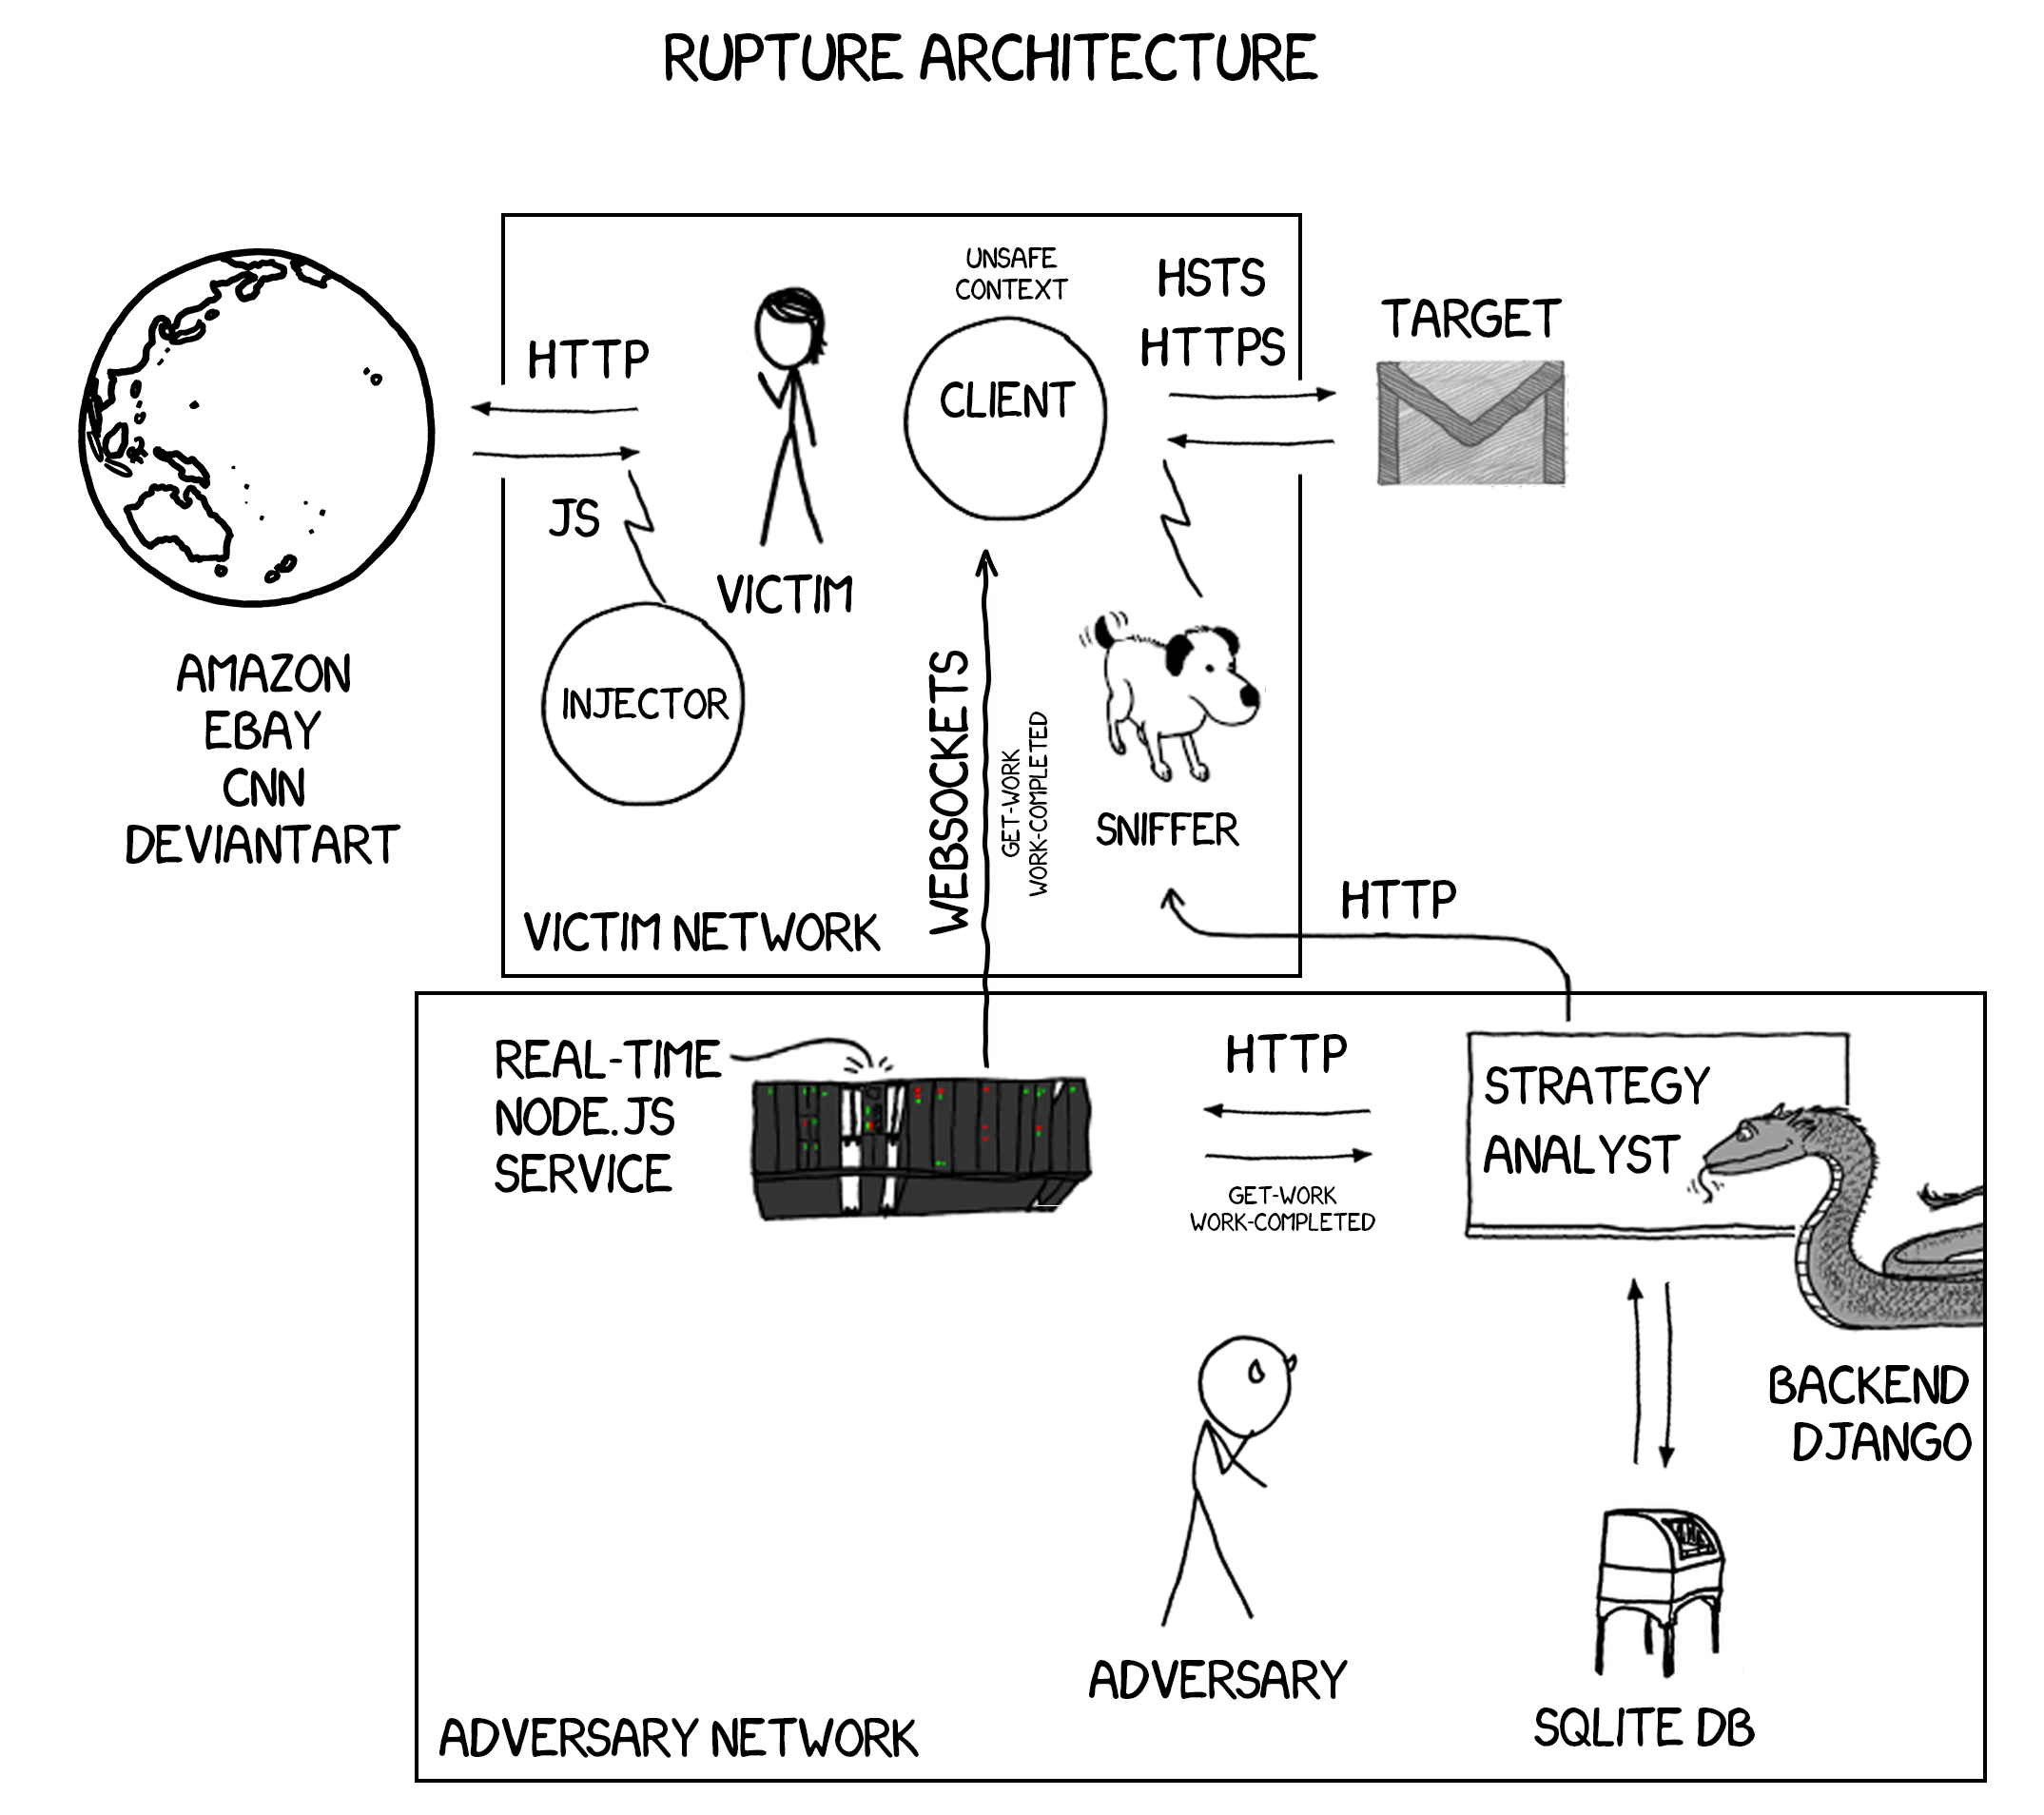
\includegraphics[width=0.48\textwidth]{architecture.png}
      \caption{Rupture Architecture}
   \end{figure}

\section{Practical optimization methods}\label{app:optimization}

\subsection{Block alignment}\label{subsec:blockalign}
Block ciphers are \textit{length monotonic}, but not \textit{strictly length
monotonic}, as described in section \ref{subsec:lenmonotone}. Specifically, the
length of the encrypted text is rounded to a product of $\mu$-bits, where $\mu$
is the block size, using added padding. The same applies for stream ciphers,
whose functionality is similar to block ciphers with block size 1 byte. In this
case, plaintext length difference between two messages does not always result in
length difference between the respective encrypted ciphertext.

It is possible to bypass this problem by using block alignment. Block alignment
techniques have already been explored in the literature \cite{c14}.  This method
demands issuing multiple requests to the reflection oracle while including
artificial noise in the reflection string $r$.  That way, one out of
$\ceil{\mu / |r^i|}$ requests, where $|r^i|$ is the length of one digit of
$r$ in bits, will result in a block distinction between different reflection
strings $r_i$.

\subsection{Reflection computation methods}\label{subsec:reflectionmethods}
Reflection strings $r$ should be polynomially computable, as defined in
\ref{sec:propertycom}. BREACH, defined in \ref{subsec:breachapp}, is
parameterized with an alphabet of ASCII symbols $\mathcal{S}$ for each character of the
secret. A successful attack should distinguish a single character of the
alphabet as the correct one through a series of requests to the reflection
oracle.

The first method of issuing requests is serial. Each request to the oracle
corresponds to a single character of the alphabet. An attack phase is completed
when requests have been issued for the entire alphabet.

In this case, $Q$ is the property "Given a known prefix $p_s$ of secret $s$ and
a symbol $t \in \mathcal{S}$, is $p_s:t$ a prefix of $s$?" and $\exists
s_i \in \mathcal{S}: Q(s_i)$ and $\forall s_j \in \mathcal{S} \setminus \{s_i\}:
\lnot Q(s_j)$. The complexity of the attack is $\mathcal{O}(|\mathcal{S}|)$ and
the round ends by finding a character of the secret.

The second method of attack is divide and conquer. In each phase the alphabet is
divided into two subsets $\mathcal{S}_1$ and $\mathcal{S}_2 = \mathcal{S}
\setminus \mathcal{S}_1$, where $|\mathcal{S}_1| = |\mathcal{S}_2| =
\ceil{|\mathcal{S}| / 2}$. The reflection string for $\mathcal{S}_1$ composes of
$|\mathcal{S}_1|$ substrings divided by an annotation symbol $\beta$. Each
substring consists of the known part of the secret concatenated with a character
in $\mathcal{S}_1$. The reflection string for $\mathcal{S}_2$ is constructed
similarly. Each phase consists of one call to the reflection oracle per subset.

Property $Q$ is defined "Given a known prefix $p_s$ of secret $s$, is $p_s:t$ a
prefix of $s$, where $t \in \mathcal{S}_1$?". As long as the prefix of the
secret is \textit{compression-detectable} by each substring of the reflection,
the end of each phase marks the choice of subset $\mathcal{S}_i$ that contains
the correct alphabet symbol and the same method is applied using chosen
$\mathcal{S}_i$ as the alphabet $\mathcal{S}$. The round is complete when
$|\mathcal{S}| = 1$. Each round reduces the alphabet by half, so the complexity
of the attack with the divide and conquer method  is
$\mathcal{O}(log_2|\mathcal{S}|)$.

\subsection{Request parallelization}\label{subsec:parallel}
The reflection oracle is generally considered as synchronous. However, this is not
always the case, since it may be able to handle multiple parallel requests from
the adversary.

This is the case for the oracle in the practical BREACH application, described
in \ref{subsec:breachapp}. In that case the reflection oracle is an endpoint
offered by a web application and the communication channel between the adversary
and the oracle is the end-to-end browser-server network channel.

Modern web servers are able to handle multiple parallel requests and
browsers can issue a certain amount of parallel requests per domain. This
functionality enables the adversary to issue multiple parallel requests per
symbol in alphabet $\mathcal{S}$ and efficiently reduce the execution time of
the attack.

\subsection{Request soup}
Previous sections demonstrated the need for multiple requests per reflection
string $r_i$. However, it is often the case that communication with the
reflection oracle given consequent analysis of each single request is time
expensive. In this case, it is preferable to issue multiple indistinguishable
requests and treat them as a set for the relative symbol.

This technique is useful in the case of the BREACH attack described in
{subsec:breachapp}. In this case, communication between the browser and the
endpoint that serves as the reflection oracle is encrypted, so the analysis of
the captured packets is time expensive per request set.

A request set consists of requests for a symbol $s_i$ in alphabet $\mathcal{S}$,
so bigger request sets result in less time delay. Length calculation per request
can then be measured as the mean length over the number of requests in the set.

This method can be combined with the methods described in \ref{subsec:parallel}
in order to utilize the parallelization and reduce the time cost of the
necessary multiple requests.

\begin{thebibliography}{13}

\bibitem{c1} J. Rizzo and T. Duong, "The CRIME attack", Ekoparty, 2012.

\bibitem{c2} Be'ery, T. and A. Shulman, "A Perfect CRIME? Only TIME Will Tell",
Black Hat Europe 2013, 2013.

\bibitem{c3} Y. Gluck, N. Harris and A. Prado, "BREACH: Reviving the CRIME attack",
Black Hat USA, 2013.

\bibitem{c4} NIST, "Announcing the ADVANCED ENCRYPTION STANDARD (AES)", 2001.

\bibitem{c5} J. Ziv and A. Lempel, "A universal algorithm for sequential data
compression", Information Theory, IEEE Transactions, vol. 23, 1977.

\bibitem{c6} J. Alawatugoda, D. Stebila and C. Boyd, "Protecting encrypted
cookies from compression side-channel attacks", 2014.

\bibitem{c7} J. Kelley and R. Tamassia, "Secure Compression: Theory \& Practice",
2014.

\bibitem{c8} M. West, "First-Party-Only Cookies", RFC Internet-Draft, 2015.

\bibitem{c9} [online] URL:
\url{https://www.facebook.com/notes/protect-the-graph/preventing-a-breach-attack/1455331811373632}
[cited May 2016]

\bibitem{c10} P. Deutsch, "DEFLATE Compressed Data Format Specification version
1.3", RFC 1951, 1996.

\bibitem{c11} [online] URL: \url{https://ruptureit.com} [cited May 2016]

\bibitem{c12} D. Karakostas and D. Zindros, "Practical New Developments on
BREACH", Black Hat Asia, 2016.

\bibitem{c13} John Kelsey, "Compression and information leakage of plaintext", 2002.

\bibitem{c14} B. Moller, T. Duong, K. Kotowicz, This POODLE Bites: Exploiting the SSL 3.0 Fallback, September 2014.

\end{thebibliography}

\end{document}
